\section{Renormalization of the MRSSM}\label{sec:renMRSSM}
This section discusses the removal of ultraviolet divergences in the amplitude of squark production at 1-loop level in the RSQCD. After an introduction and discussion of the regularization schemes, field and mass renormalization constants are calculated in dimensional regularization in the on-shell scheme. After that the renormalization constant of the strong gauge coupling $g_s$ is computed in a mixture of $\overline{\mathrm{MS}}$- and zero-momentum subtraction scheme. This was done because the gauge coupling of the parton density functions is given in the $\overline{\mathrm{MS}}$-scheme but does not include heavy particles, such as the top-quark or supersymmetric particles in its $\beta$-function. However renormalizing these heavy particles in the zero-momentum subtraction implies that the $\beta$-function of $g_s$ is exactly the one from QCD. This is shown in section \ref{sec:beta_function}. After that a fact already discussed in section \ref{sec:RegSchemeDep} is revisited: the used regularization breaks supersymmetry. Section \ref{sec:SUSYrestore} describes the calculation of an extra counterterm which restores supersymmetry. Finally the UV-divergent parts of all renormalization constants in the RSQCD are given. These might prove useful when someone is to check for UV-finiteness of a Green-function or a physical observable. The chapter closes with a discussion of the renormalizes matrix amplitude.
%In order to improve the prediction of cross sections one has to take quantum corrections into account. These are associated with loops in the corresponding Feynman diagrams. Computing these loop diagrams one might encounter infinities which arise from certain momentum configurations of the unspecified loop momenta. These infinities can be classified due to their origin. Infinities which are associated with loop momenta which tend to infinity are referred to as ultraviolet(UV) divergences. Infinities arising from loop momenta approaching zero can occur in loops with massless particles and are called infrared(IR) singularities. \\%Furthermore there are collinear singularities with occur when a massless particle splits into two massless collinear particles.\\
%These infinities are not physical and must therefore be removed to get sensible predictions. To this end one regularizes them to extract them from the quantity in question. UV-divergences can be removed by means of renormalization, i.e. counterterms are inserted into the Lagrangian to cancel UV-divergences. Infrared and collinear divergenves are removed by adding up all possible contributions which give rise to the considered observable.

\subsection{Regularization Schemes}\label{sec:RegSchemes}
\subsubsection*{Dimensional Regularization (DREG)}
Dimensional regularization(DREG) is a very common procedure for regularizing infinities which was devised by t'Hooft and Veltman~\cite{'tHooft:1972fi}. In this scheme loop momenta, gamma- and epsilon-tensors, phase space and fields are defined in $D$ dimensions. As in every regularization scheme a parameter with mass dimension needs to be introduced. In DREG that is the $\mu$ parameter which ensures that the loop integrals still have mass dimension 4:
\begin{align}
\int \frac{\mbox{d}^4p}{(2\pi)^4} \to \mu^{4-D} \int \frac{\mbox{d}^Dp}{(2\pi)^D}.
\end{align}
One often writes $D=4-2\epsilon$. Then the divergences of the loop integral manifest in $\frac{1}{\epsilon}$ poles.\\
However DREG suffers a flaw in supersymmetry. As the degrees of freedom of a massless gauge boson are $D-2$ but the degrees of freedom of its superpartner are 2 there is a mismatch if $D \neq 4$. As a consequence there are $2\epsilon$ degrees of freedom associated with the gluon\footnote{These degrees of freedom are identified with scalars and are therefore referred to as $\epsilon$ scalars} which do not have a supersymmetric partner. Therefore DREG violates supersymmetry.

\subsubsection*{Dimensional Reduction (DRED)}
Dimensional reduction (DRED) was introduced to rectify the imperfections of DREG, i.e. it preserves supersymmetry\footnote{It is not clear if DRED preserves supersymmetry at all orders in perturbation theory but it does preserve supersymmetry at the 1-loop level.}. DRED promotes only loop momenta to $D$ dimensions. All other quantities which are $D$ dimensional in DREG stay in 4 dimensions.\\
maybe refer to Collins: Renormalization


\subsection{Regularization Scheme Dependences}\label{sec:RegSchemeDep}
To discuss the subject of this and ensuing subsections it is useful to introduce the effective action $\Gamma$. A formal introduction of $\Gamma$ can be found in~\cite{Peskin}. In short $\Gamma$ can be viewed as a modification of the classical action $\Gamma_{\mathrm{cl}} = \int \mathcal{L}_{\mathrm{cl}}$ by quantum effects:
\begin{align}
\Gamma = \Gamma_{\mathrm{cl}} + \mathcal{O}(\hbar)
\end{align}
This means that in addition to the vertices in the classical Lagrangian new vertices arise due to loop effects. As already alluded to loop corrections might a priori not be finite and then need to be rendered finite by the addition of counterterms. For $\mathcal{O}(\hbar)$ corrections one writes
\begin{align}
\Gamma^{(\leq 1)} \to \Gamma^{(\leq 1)} + \Gamma^{(1),\ \mathrm{ct}}
\end{align} 
These counterterms depend on the regularization (and renormalization) scheme. If one chooses to work with DREG supersymmetry will not be preserved at 1-loop order, i.e. $\Gamma^{(\leq 1)}_{\mathrm{DREG}}$ is not supersymmetric. To maintain supersymmetry invariance of the renormalized effective action the counterterms will not only consist of supersymmetric counterterms $\Gamma^{(1),\ \mathrm{ct,\ sym}}_{\mathrm{DREG}}$ but also of counterterms restoring supersymmetry $\Gamma^{(1),\ \mathrm{ct,\ trans}}_{\mathrm{DREG}}$. 
\begin{align}
\Gamma^{(1),\ \mathrm{ct}}_{\mathrm{DREG}} = \Gamma^{(1),\ \mathrm{ct,\ sym}}_{\mathrm{DREG}} + \Gamma^{(1),\ \mathrm{ct,\ trans}}_{\mathrm{DREG}}
\end{align}
Fortunately a supersymmetry conserving regularization scheme (at 1-loop level) is given by DRED \cite{Hollik:2001cz}. One way to acquire supersymmetry restoring counterterms is therefore given by
\begin{align}
\Gamma^{(\leq 1)}_{\mathrm{DRED}} + \Gamma^{(1),\ \mathrm{ct}}_{\mathrm{DRED}} \overset{!}{=} \Gamma^{(\leq 1)}_{\mathrm{DREG}} + \Gamma^{(1),\ \mathrm{ct}}_{\mathrm{DREG}}.
\end{align}
Equating also the finite terms in $\Gamma^{(1),\ \mathrm{ct,\ sym}}$ in DRED and DREG the choice of the supersymmetry restoring counterterms is fixed by\cite{Varso}:
\begin{align}
\Gamma^{\mathrm{(1),ct,trans}}_{\mathrm{DREG}} = \Gamma^{(\leq 1)}_{\mathrm{DRED}} - \Gamma^{(\leq 1)}_{\mathrm{DREG}}.\label{eq:GammaCtRestore}
\end{align} 
This equation justifies the label "trans" at the supersymmetry restoring counterterm because it actually describes the transition counterterm from DREG to DRED or vice versa.\\ %This way supersymmetry is preserved by the renormalization constants.\\ 
In the case of the MRSSM it will turn out that the only supersymmetry violation comes from corrections associated with the gluon as already alluded to in section \ref{sec:RegSchemes}. However supersymmetry restoring will always already be included in $\delta Z^{\mathrm{DREG}}$. Referring to the field renormalization constants from eq. \ref{eq:fieldtrafo} this is 
\begin{align}
\delta Z^{\mathrm{DREG}} = \delta Z^{\mathrm{DREG,sym}} + \delta Z^{\mathrm{trans}}
\end{align}
where 
\begin{align}
\delta Z^{\mathrm{trans}} = \delta Z^{\mathrm{DREG}} - \delta Z^{\mathrm{DRED}}
\end{align}
is the supersymmetry restoring renormalization constant. Note the sign within this definition in comparison to eq. \ref{eq:GammaCtRestore}. The only point where particularly care is required is the coupling: The  gauge coupling $g_s$ and the Yukawa coupling $\hat{g}_s$ receive different supersymmetry restoring counterterms due to different loop diagrams. Therefore one has to make a difference between these couplings at 1-loop level. In order to match $g_s$ to the experimentally measured coupling it is renormalized in the  $\overline{\mathrm{MS}}$-scheme (with an additional manipulation for heavy particles, which will be explained in subsection \ref{sec:RenGaugeCoupling}). The Yukawa coupling $\hat{g}_s$ therefore needs to be added with the difference of the supersymmetry restoring counterterms from the $q\tilde{q}^\dagger\tilde{g}$ vertex and the $q\overline{q}G$ vertex at 1-loop in order to be renormalized in the same way.


%An alternative procedure is used in \cite{Beenakker:1996ch}, where only one supersymmetry restoring counterterm, which translates between the renormalized gauge coupling $g_s$ and the renormalized Yukawa coupling $\hat{G}_s$ is needed. That is possible because the only supersymmetry violation comes from the gauge sector. For a comprehensive discussion of this issue see [Philipp Vasros Diplomarbeit and the paper with Dominik]\\
%SUSY restoring is always already in $\delta Z^{DREG}$ included. Only important thing is the coupling: $g_s$ and $\hat{g}_s$ receive different SUSY restoring counterterm. Therefore one has to make a difference between these couplings at 1-loop level. In order to match $g_s$ to the experimentaly measured coupling it is renormalized in $\overline{\mathrm{MS}}$. The Yukawa coupling $\hat{g}_s$ therefore needs to be added with the difference of the SUSY-restoring counterterms at 1-loop in order to be renormalized the same way.


\subsection{On-Shell Renormalization}\label{sec:QuarkSE}
A part of the computation of the cross section at next-to-leading order is the calculation of renormalization constants. 
Field renormalization constants $\delta Z$ and parameter renormalization constants $\delta o$ with $o \in \left\{ g, m \right\}$ are defined by
\begin{align}
Z = 1 + \delta Z \hspace{3cm} o_{\mathrm{bare}} = o + \delta o
\end{align}
where $Z$ and $o$ are defined by the multiplicative renormalization transformation, introduced in eq. \ref{eq:fieldtrafo} and \ref{eq:fieldtrafo}. The field and mass renormalization constants have been calculated in DREG in the on-shell scheme. This has the advantage that when turning to the cross section no manipulation of the Green function to the S-matrix element has to be done, see section \ref{sec:LSZ}.\\
The calculation has partially been performed by hand but was always checked with the mathematica output generated by the packages  \texttt{FeynArts} \cite{Hahn:2000} and \texttt{FormCalc} \cite{ChokoufeNejad:2013qja, Hahn:1998yk}.

\subsubsection*{The Quark Self-Energy}
The quark self-energy splits into contribution from the Standard Model as well as a supersymmetric analogue which is already present in the MSSM.
\begin{figure}[!htbp]
\begin{center}
\begin{tikzpicture}[line width=1.5 pt, scale=1.3]
	\draw[fermionbar](180:1.3)--(180:0.5);
	\draw[fermionnoarrow] (-0.5,0) arc (180:0:.5);
	\draw[fermionnoarrow] (0.5,0) arc (0:-180:.5);	
	\node at (0,0) {1L};
	\draw[fermionbar](0:0.5)--(0:1.3);
	\node at (1.8,0) {=};
\begin{scope}[shift={(3.5,0)}]
	\draw[fermionbar](180:1.3)--(180:0.5);
	\draw[gluon] (-0.5,0) arc (180:0:.5);
	\node at (0,0.8) {$G$};
	\draw[fermion] (0.5,0) arc (0:-180:.5);
	\node at (0,-0.8) {$q$};	
	\draw[fermionbar](0:0.5)--(0:1.3);
	\node at (1.8,0) {+};
\end{scope}
\begin{scope}[shift={(7,0)}]
	\draw[fermionbar](180:1.3)--(180:0.5);
	\draw[gluon] (-0.5,0) arc (180:0:.5);
	\draw[fermionnoarrow] (-0.5,0) arc (180:0:.5);
	\node at (0,0.8) {$\tilde{g}$};
	\draw[scalar] (0.5,0) arc (0:-180:.5);
	\node at (0,-0.8) {$\tilde{q}$};	
	\draw[fermionbar](0:0.5)--(0:1.3);
\end{scope}
\end{tikzpicture}
\caption{Feynman diagrams contributing to the self-energy of the quark at 1-loop level.}\label{fig:QuarkSelfEnergy}
\end{center}
\end{figure}\\
The one-particle-irreducible diagrams evaluate to
\begin{align}
i\Gamma^{\mathrm{1L}}_{q_i\overline{q}_j} = i \frac{g_s^2}{16\pi^2}\delta_{ij} C(F) \left[ 2 \left( B_0(p^2,0,0) + B_1(p^2,0,0)-\frac{1}{2}\right)\slashed{p} - 2 B_1(p^2,m_{\tilde{g}}^2,m_{\tilde{q}}^2)\slashed{p}\right].\label{eq:QuarkSE}
\end{align}
With the counterterm Feynman rule\\
\\
\begin{tikzpicture}[line width=1.0 pt, scale=0.8]
	\node at (-2.5,-0.1) {$i\Gamma^{\mathrm{1L,ct}}_{q_i\overline{q}_j}\ \hat{=}\ i$};
\begin{scope}[shift={(0.1,0)}]	
	\draw[fermionbar] (-1.3,0) --(0,0);
	\draw[fermionnoarrow] (-0.3,0.3) -- (0.3,-0.3);
	\draw[fermionnoarrow] (-0.3,-0.3) -- (0.3,0.3);
	\draw[fermionbar] (0,0) --(1.3,0);
	\node at (1.6,-0.1) {$j$};
	\node at (3,0) {$\hat{=}\ i\delta_{ij}\delta Z_q \slashed{p} $};	
\end{scope}
\end{tikzpicture}\\
and the on-shell renormalization condition
\begin{align}
\frac{\partial}{\partial \slashed{p}} \left[ \Re (\Gamma^{\mathrm{1L}}_{q_i\overline{q}_j}) + \Gamma^{\mathrm{1L,ct}}_{q_i\overline{q}_j}  \right]_{p^2 = 0} = 0
\end{align}
where $\Re (\hdots)$ denotes the real part of $\hdots$ one finds
\begin{align}
\delta Z_q = 2 C(F) \frac{g_s^2}{16\pi^2} \Re \left[ B_1(0 ,m_{\tilde{g}}^2,m_{\tilde{q}}^2) \right].
\end{align}
Note that the Standard Model contribution to the quark renormalization constant equals zero as it is propotional to $B_0(0,0,0)$ and $B_1(0,0,0)$. These integrals have no mass scale and are due to their definition of their scaling in $D$ dimensions\cite{Collins:105730} defined to be zero. Pictorially this may be understood as a cancellation of a positive UV-divergent part and a negative IR-divergent part. Note further that the term $\frac{1}{2}$ from eq. \ref{eq:QuarkSE} has vanished because it has been absorbed in $B_0(p^2,0,0)|_{p^2 \to 0}$.\\
Doing the same calculation in DRED one finds that this very term $\frac{1}{2}$ is absent. Therefore the transition renormalization constant between DREG and DRED is given by
\begin{align}
\delta Z_q^{\mathrm{trans}} = \delta Z_q^{\mathrm{DREG}} - \delta Z_q^{\mathrm{DRED}} = C(F) \frac{g_s^2}{16\pi^2}.\label{eq:QuarkSC}
\end{align}

\subsubsection*{The Squark Self-Energy}
The contributions to the self-energy of the left- and right-handed squark are the same for electroweak effects are neglected. Therefore to avoid unnecessary labeling $\Gamma_{\tilde{q}\tilde{q}^\dagger}$ stands in the following for $\Gamma_{\tilde{q}_L\tilde{q}_L^\dagger} = \Gamma_{\tilde{q}_R\tilde{q}_R^\dagger}$.
\begin{figure}[!htbp]
\begin{center}
\begin{tikzpicture}[line width=1.5 pt, scale=1.3]
	\draw[scalarbar](180:1.3)--(180:0.5);
	\draw[fermionnoarrow] (-0.5,0) arc (180:0:.5);
	\draw[fermionnoarrow] (0.5,0) arc (0:-180:.5);	
	\node at (0,0) {1L};
	\draw[scalarbar](0:0.5)--(0:1.3);
	\node at (1.8,0) {=};
\begin{scope}[shift={(3.5,0)}]
	\draw[scalarbar](-1.3,0)--(0,0);
	\draw[scalarbar](0,0)--(1.3,0);
	\draw[scalar] (0,0) arc (-90:270:.5);
	\node at (0,1.3) {$\tilde{q}$};
	\node at (1.8,0) {+};
\end{scope}
\begin{scope}[shift={(7.0,0)}]
	\draw[scalarbar](-1.3,0)--(0,0);
	\draw[scalarbar](0,0)--(1.3,0);
	\draw[gluon] (0,0) arc (270:-90:.5);
	\node at (0,1.3) {$G$};
	\node at (1.8,0) {+};
\end{scope}
\begin{scope}[shift={(10.5,0)}]
	\draw[scalarbar](180:1.3)--(180:0.5);
	\draw[gluon] (-0.5,0) arc (180:0:.5);
	\draw[fermionnoarrow] (-0.5,0) arc (180:0:.5);
	\node at (0,0.8) {$\tilde{g}$};
	\draw[fermion] (0.5,0) arc (0:-180:.5);
	\node at (0,-0.8) {$q$};	
	\draw[scalarbar](0:0.5)--(0:1.3);
\end{scope}
\begin{scope}[shift={(3.5,-2.5)}]
	\node at (-1.8,0) {+};
	\draw[scalarbar](180:1.3)--(180:0.5);
	\draw[scalarnoarrow] (-0.5,0) arc (180:0:.5);
	\node at (0,0.8) {$\phi^0,\ \sigma^0$};
	\draw[scalar] (0.5,0) arc (0:-180:.5);
	\node at (0,-0.8) {$\tilde{q}$};	
	\draw[scalarbar](0:0.5)--(0:1.3);
	\node at (1.8,0) {+};
\end{scope}
\begin{scope}[shift={(7,-2.5)}]
	\draw[scalarbar](180:1.3)--(180:0.5);
	\draw[gluon] (-0.5,0) arc (180:0:.5);
	\node at (0,0.8) {$G$};
	\draw[scalar] (0.5,0) arc (0:-180:.5);
	\node at (0,-0.8) {$\tilde{q}$};	
	\draw[scalarbar](0:0.5)--(0:1.3);
\end{scope}
\end{tikzpicture}
\caption{Diagrammatic contributions to the self-energy of the squark at 1-loop level.}
\end{center}
\end{figure}\\
\begin{align}
i\Gamma^{\mathrm{1L}}_{\tilde{q}_{i}\tilde{q}^\dagger_j} &= i \frac{g_s^2}{16\pi^2}\delta_{ij}C(F) \left[  A_0(m_{\tilde{q}}^2) + 0 - \left( 4A_0(m_{\tilde{g}}^2) + 4B_1(p^2,0,m_{\tilde{g}}^2)p^2 \right) \right.\nonumber\\
& \left.+ 4m_{\tilde{g}}^2B_0(p^2,m_{\phi^0}^2,m_{\tilde{q}}^2) - \left(2B_1(p^2,0,m_{\tilde{q}}^2)p^2 + B_0(p^2,0,m_{\tilde{q}}^2)(m_{\tilde{q}}^2+3p^2) \right) \right].
\end{align}
Suppressing $\delta_{AB}$ with $A,B \in \left\{ L,R \right\}$ which is present in the tree level propagator (see fig. \ref{fig:firstFeynmanRules}) the counterterm Feynman rule is given by\\
\\
\begin{tikzpicture}[line width=1.0 pt, scale=0.8]
	\node at (-2.5,-0.1) {$i\Gamma^{\mathrm{1L,ct}}_{q_i\overline{q}_j}\ \hat{=}\ i$};
\begin{scope}[shift={(0.1,0)}]	
	\draw[scalarbar] (-1.3,0) --(0,0);
	\draw[fermionnoarrow] (-0.3,0.3) -- (0.3,-0.3);
	\draw[fermionnoarrow] (-0.3,-0.3) -- (0.3,0.3);
	\draw[scalarbar] (0,0) --(1.3,0);
	\node at (1.6,-0.1) {$j$};
	\node at (5.1,0) {$\hat{=}\ i\delta_{ij} \left[ \delta Z_{\tilde{q}}(p^2-m_{\tilde{q}}^2) - \delta m_{\tilde{q}}^2 \right] .$};	
\end{scope}
\end{tikzpicture}\\
The on-shell renormalization conditions read
\begin{align}
&\frac{\partial}{\partial p^2} \left[ \Re (\Gamma^{\mathrm{1L}}_{\tilde{q}_{i}\tilde{q}^\dagger_j}) + \Gamma^{\mathrm{1L,ct}}_{\tilde{q}_{i}\tilde{q}^\dagger_j}  \right]_{p^2 = m_{\tilde{q}}^2} = 0 && \left[ \Re (\Gamma^{\mathrm{1L}}_{\tilde{q}_{i}\tilde{q}^\dagger_j}) + \Gamma^{\mathrm{1L,ct}}_{\tilde{q}_{i}\tilde{q}^\dagger_j}  \right]_{p^2 = m_{\tilde{q}}^2} = 0.
\end{align}
This results in the following renormalization constants
\begin{align}
\delta Z_{\tilde{q}} &= \frac{g_s^2}{16\pi^2}C(F) \Re \left[ 4B_1(p^2,0,m_{\tilde{g}}^2) + 2B_1(B_1(p^2,0,m_{\tilde{q}}^2)) + 3B_0(p^2,0,m_{\tilde{q}}^2) \right.\nonumber\\
& + 4m_{\tilde{q}}^2 \frac{\partial}{\partial p^2}B_1(p^2,0,m_{\tilde{g}}^2) - 4m_{\tilde{g}}^2\frac{\partial}{\partial p^2}B_0(p^2,m_{\phi^0}^2,m_{\tilde{q}}^2) + 2m_{\tilde{q}}^2 \frac{\partial}{\partial p^2}B_1(p^2,0,m_{\tilde{q}}^2)\nonumber\\
& \left. + 4m_{\tilde{q}}^2 \frac{\partial}{\partial p^2}B_0(p^2,0,m_{\tilde{q}}^2)\right]_{p^2 = m_{\tilde{q}}^2}
\end{align}
and
\begin{align}
\delta m_{\tilde{q}}^2 = \frac{g_s^2}{16\pi^2}C(F)&\left[ A_0(m_{\tilde{q}}^2) - (4A_0(m_{\tilde{g}}^2) + 4B_1(m_{\tilde{q}}^2,0,m_{\tilde{g}}^2)m_{\tilde{q}}^2) + 4 m_{\tilde{g}}^2 B_0(m_{\tilde{q}}^2,m_{\phi^0}^2,m_{\tilde{q}}^2) \right.\nonumber\\
&\left. -(2B_1(m_{\tilde{q}}^2,0,m_{\tilde{q}}^2) m_{\tilde{q}}^2 + 4 B_0(m_{\tilde{q}}^2,0,m_{\tilde{q}}^2)m_{\tilde{q}}^2) \right].
\end{align}
The squark self-energy exhibits no regularization dependence. The transition counterterms are therefore 
\begin{align}
\delta Z_{\tilde{q}}^{\mathrm{trans}} = \delta m_{\tilde{q}}^{2\ \mathrm{trans}} = 0. \label{eq:SquarkSC}
\end{align}

\subsubsection*{The Glunio Self-Energy}
The 4-spinor of the gluino comprises two Weyl spinors which describe very different particles.
\begin{align}
\tilde{g}^a = \begin{pmatrix}
-i\lambda^a \\
i\overline{\chi}^a
\end{pmatrix}
\end{align}
The left-handed part $\lambda^a$ is associated with the superpartner of the gluon and therefore the "actual" gluino whereas the right-handed part $\overline{\chi}^a$ was introduced to assign a Dirac-mass to the gluino and may be referred to as the octino.\\
From the Lagrangian \ref{eq:L_RSQCD} one can see that the couplings of the two particles are quite distinct. This is reflected by different field renormalization constants of the left- and right-handed part of the gluino.
\begin{figure}[!htbp]
\begin{center}
\begin{tikzpicture}[line width=1.5 pt, scale=1.3]
	\draw[fermionnoarrow](180:1.3)--(180:0.5);
	\draw[gluon](180:1.3)--(180:0.5);
	\draw[fermionnoarrow] (-0.5,0) arc (180:0:.5);
	\draw[fermionnoarrow] (0.5,0) arc (0:-180:.5);	
	\node at (0,0) {1L};
	\draw[fermionnoarrow](0:0.5)--(0:1.3);
	\draw[gluon](0:0.5)--(0:1.3);
	\node at (1.8,0) {=};
\begin{scope}[shift={(3.5,0)}]
	\draw[fermionnoarrow](180:1.3)--(180:0.5);
	\draw[gluon](180:1.3)--(180:0.5);
	\draw[fermionbar] (-0.5,0) arc (180:0:.5);
	\node at (0,0.8) {$q$};
	\draw[scalarbar] (0.5,0) arc (0:-180:.5);
	\node at (0,-0.8) {$\tilde{q}$};	
	\draw[fermionnoarrow](0:0.5)--(0:1.3);
	\draw[gluon](0:0.5)--(0:1.3);
	\node at (1.8,0) {+};
\end{scope}
\begin{scope}[shift={(7.0,0)}]
	\draw[gluon](180:1.3)--(180:0.5);
	\draw[fermionnoarrow](180:1.3)--(180:0.5);
	\draw[scalarnoarrow] (-0.5,0) arc (180:0:.5);
	\node at (0,0.8) {$\phi^0,\sigma^0$};
	\draw[fermionnoarrow] (0.5,0) arc (0:-180:.5);
	\draw[gluon] (0.5,0) arc (0:-180:.5);
	\node at (0,-0.8) {$\tilde{g}$};	
	\draw[gluon](0:0.5)--(0:1.3);
	\draw[fermionnoarrow](0:0.5)--(0:1.3);
	\node at (1.8,0) {+};
\end{scope}
\begin{scope}[shift={(10.5,0)}]
	\draw[gluon](180:1.3)--(180:0.5);
	\draw[fermionnoarrow](180:1.3)--(180:0.5);
	\draw[gluon] (-0.5,0) arc (180:0:.5);
	\node at (0,0.8) {$G$};
	\draw[fermionnoarrow] (0.5,0) arc (0:-180:.5);	
	\draw[gluon] (0.5,0) arc (0:-180:.5);
	\node at (0,-0.8) {$\tilde{g}$};	
	\draw[fermionnoarrow](0:0.5)--(0:1.3);
	\draw[gluon](0:0.5)--(0:1.3);
\end{scope}
\end{tikzpicture}
\caption{diagrammatic contributions to the self-energy of the squark at 1-loop level}
\end{center}
\end{figure}
As for the quarks the fermion (and momentum) flow is from the right to the left.
\begin{align}
i\Gamma^{1L}_{\tilde{g}^a \overline{\tilde{g}}^b} &= i \frac{g_s^2}{16\pi^2}\delta_{ab} \left[-4T(F)\left( (n_f-1) B_1(p^2,0,m_{\tilde{q}}^2) + B_1(p^2,m_t^2,m_{\tilde{q}}^2) \right)P_L \slashed{p} \right.\nonumber\\
& + C(A)\left( (B_0(p^2,m_{\tilde{g}}^2,m_{\phi^0}^2) - B_0(p^2,m_{\tilde{g}}^2,m_{\sigma^0}^2))m_{\tilde{g}} - (B_1(p^2,m_{\tilde{g}}^2,m_{\phi^0}^2) + B_1(p^2,m_{\tilde{g}}^2,m_{\sigma^0}^2))\slashed{p} \right) \nonumber\\
&\left.+ C(A)\left( (2 - 4 B_0(p^2,0,m_{\tilde{g}}^2)) m_{\tilde{g}} - (1-2(B_0(p^2,0,m_{\tilde{g}}^2) + B_1(p^2,0,m_{\tilde{g}}^2)))\slashed{p} \right)\right]
\end{align}
Where $n_f = 6$ is the number of quark flavors.\\
The counterterm Feynman rule derived from multiplicative renormalization reads\\
\begin{tikzpicture}[line width=1.0 pt, scale=0.8]
	\node at (-2.5,-0.1) {$i\Gamma^{1L,ct}_{\tilde{g}^a \overline{\tilde{g}}^b}\ \hat{=}\ a$};
\begin{scope}[shift={(0.1,0)}]	
	\draw[gluon] (-1.3,0) --(1.3,0);
	\draw[fermionnoarrow] (-0.3,0.3) -- (0.3,-0.3);
	\draw[fermionnoarrow] (-0.3,-0.3) -- (0.3,0.3);
	\draw[fermionnoarrow] (-1.3,0) --(1.3,0);
	\node at (1.6,0) {$b$};
	\node at (7.8,0) {$\hat{=}\ i\delta_{ab}\left[ (\delta Z_{\tilde{g}}^L P_L + \delta Z_{\tilde{g}}^R P_R)\slashed{p} - \left(\frac{\delta Z_{\tilde{g}}^L+\delta Z_{\tilde{g}}^R}{2} m_{\tilde{g}} +\delta m_{\tilde{g}}\right) \right]. $};	
\end{scope}
\end{tikzpicture}\\
The on-shell renormalization conditions for the fields are
\begin{align}
& \frac{\partial}{\partial (P_L\slashed{p})} \left[ \Re (\Gamma^{\mathrm{1L}}_{\tilde{g}^a \overline{\tilde{g}}^b}) + \Gamma^{\mathrm{1L,ct}}_{\tilde{g}^a \overline{\tilde{g}}^b}  \right]_{\slashed{p} = m_{\tilde{g}}} = 0,
&& \frac{\partial}{\partial (P_R\slashed{p})} \left[ \Re (\Gamma^{\mathrm{1L}}_{\tilde{g}^a \overline{\tilde{g}}^b}) + \Gamma^{\mathrm{1L,ct}}_{\tilde{g}^a \overline{\tilde{g}}^b}  \right]_{\slashed{p} = m_{\tilde{g}}} = 0
\end{align}
where the derivative of $\Sigma = \Sigma^{VL}P_L\slashed{p} + \Sigma^{VR}P_R\slashed{p} + \Sigma^{SL}P_L + \Sigma^{SR}P_R$ with respect to $P_A\slashed{p}$ \\
($A \in \left\{ L,R \right\}$) is defined by\cite{FormCalcManual}
\begin{align}
\left.\frac{\partial}{\partial (P_A\slashed{p})} \Sigma\right|_{\slashed{p} = m} = \Sigma^{VA} + \frac{\partial}{\partial p^2} \left( m^2 \Sigma^{VL} + m^2 \Sigma^{VR} + m \Sigma^{SL} + m \Sigma^{SR}\right).
\end{align}
This leads to the following renormalization constants
\begin{align}
\delta Z_{\tilde{g}}^L &= \frac{g_s^2}{16\pi^2}\Re \left[ 4T(F)\left( (n_f-1) B_1(m_{\tilde{g}}^2,0,m_{\tilde{q}}^2) + B_1(m_{\tilde{g}}^2,m_t^2,m_{\tilde{q}}^2) \right) \right.\nonumber\\
&+C(A) (B_1(m_{\tilde{g}}^2,m_{\tilde{g}}^2,m_{\phi^0}^2) + B_1(m_{\tilde{g}}^2,m_{\tilde{g}}^2,m_{\sigma^0}^2))\nonumber\\
&+C(A)(1-2(B_0(m_{\tilde{g}}^2,0,m_{\tilde{g}}^2) + B_1(m_{\tilde{g}}^2,0,m_{\tilde{g}}^2)))\nonumber\\
&+ 4T(F) m_{\tilde{g}}^2 \frac{\partial}{\partial p^2} \left( ((n_f-1))  B_1(p^2,0,m_{\tilde{q}}^2) +  B_1(p^2,m_t^2,m_{\tilde{q}}^2) \right)\nonumber\\
&-2 C(A) m_{\tilde{g}} \frac{\partial}{\partial p^2} \left( B_0(p^2,m_{\tilde{g}}^2,m_{\phi^0}^2)-B_0(p^2,m_{\tilde{g}}^2,m_{\sigma^0}^2) - B_1(p^2,m_{\tilde{g}}^2,m_{\phi^0}^2) - B_1(p^2,m_{\tilde{g}}^2,m_{\sigma^0}^2) \right)\nonumber\\
&-4 C(A) m_{\tilde{g}}^2 \frac{\partial}{\partial p^2} \left.\left( -B_0(p^2,0,m_{\tilde{g}}^2) + B_0(p^2,0,m_{\tilde{g}}^2) \right)\right]_{p^2=m_{\tilde{g}}^2}
\end{align}
and 
\begin{align}
\delta Z_{\tilde{g}}^R &= \frac{g_s^2}{16\pi^2}\Re \left[C(A) (B_1(m_{\tilde{g}}^2,m_{\tilde{g}}^2,m_{\phi^0}^2) + B_1(m_{\tilde{g}}^2,m_{\tilde{g}}^2,m_{\sigma^0}^2)) \right.\nonumber\\
&+C(A)(1-2(B_0(m_{\tilde{g}}^2,0,m_{\tilde{g}}^2) + B_1(m_{\tilde{g}}^2,0,m_{\tilde{g}}^2)))\nonumber\\
&+ 4T(F) m_{\tilde{g}}^2 \frac{\partial}{\partial p^2} \left( ((n_f-1))  B_1(p^2,0,m_{\tilde{q}}^2) +  B_1(p^2,m_t^2,m_{\tilde{q}}^2) \right)\nonumber\\
&-2 C(A) m_{\tilde{g}} \frac{\partial}{\partial p^2} \left( B_0(p^2,m_{\tilde{g}}^2,m_{\phi^0}^2)-B_0(p^2,m_{\tilde{g}}^2,m_{\sigma^0}^2) - B_1(p^2,m_{\tilde{g}}^2,m_{\phi^0}^2) - B_1(p^2,m_{\tilde{g}}^2,m_{\sigma^0}^2) \right)\nonumber\\
&-4 C(A) m_{\tilde{g}}^2 \frac{\partial}{\partial p^2} \left.\left( -B_0(p^2,0,m_{\tilde{g}}^2) + B_0(p^2,0,m_{\tilde{g}}^2) \right)\right]_{p^2=m_{\tilde{g}}^2}.
\end{align}
As for the quark there are constant terms amid the Passarino-Veltman integrals. These arise only in DREG but and not in DRED. The transition counterterms are
\begin{align}
\delta Z_{\tilde{g}}^{A\ \mathrm{trans}} = \delta Z_{\tilde{g}}^{A\ \mathrm{DREG}} - \delta Z_{\tilde{g}}^{A\ \mathrm{DRED}} = C(A) \frac{g_s^2}{16\pi^2}\label{eq:GluinoSC}
\end{align}
for $A \in \left\{L,R\right\}$. The gluino mass counterterm is ascertained by the condition
\begin{align}
\left[ \Re (\Gamma^{\mathrm{1L}}_{\tilde{g}^a \overline{\tilde{g}}^b}) + \Gamma^{\mathrm{1L,ct}}_{\tilde{g}^a \overline{\tilde{g}}^b}  \right]_{\slashed{p} = m_{\tilde{g}}} = 0
\end{align}
which is equivalent to 
\begin{align}
\delta m_{\tilde{g}} = \Re\left( m_{\tilde{g}}\frac{\Sigma^{VL}+\Sigma^{VR}}{2} + \frac{\Sigma^{SL}+\Sigma^{SR}}{2} \right)
\end{align}
and yields
\begin{align}
\delta m_{\tilde{g}} &= \frac{g_s^2}{16\pi^2} m_{\tilde{g}}^2\ \Re \left[ -2T(F) \left( (n_f-1)B_1(m_{\tilde{g}}^2,0,m_{\tilde{q}}^2) + B_1(m_{\tilde{g}}^2,m_t^2,m_{\tilde{q}}^2) \right) \right.\nonumber\\
& + C(A) \left( B_0(m_{\tilde{g}}^2,m_{\tilde{g}}^2,m_{\phi^0}^2) - B_0(m_{\tilde{g}}^2,m_{\tilde{g}}^2,m_{\sigma^0}^2) - B_1(m_{\tilde{g}}^2,m_{\tilde{g}}^2,m_{\phi^0}^2) -
B_1(m_{\tilde{g}}^2,m_{\tilde{g}}^2,m_{\sigma^0}^2) \right)\nonumber\\
& + C(A) \left.\left( 1 - 2 B_0(m_{\tilde{g}}^2,0,m_{\tilde{g}}^2) + 2 B_1(m_{\tilde{g}}^2,0,m_{\tilde{g}}^2) \right)\right].
\end{align}
Again there is a transition counterterm 
\begin{align}
\delta m_{\tilde{g}}^{\mathrm{trans}} = \delta m_{\tilde{g}}^{\mathrm{DREG}} - \delta m_{\tilde{g}}^{\mathrm{DRED}} = C(A) \frac{g_s^2}{16\pi^2} m_{\tilde{g}}.
\end{align}
Apart from the renormalization constant of the gauge coupling and the supersymmetry restoring counterterm these are all renormalization constants needed from squark production at next to leading order. In fact the field renormalization constants of the gluino are not needed as they drop out when summing up all three counterterm Feynman diagrams. This can be seen when writing down the matrix amplitudes for the counterterm Feynman diagrams shown in fig. \ref{fig:CounterTerm}:
\begin{align}
\mathcal{M}^{\mathrm{B}} &= -2g_s^2 \frac{\left\langle v_2 |P_R \slashed{k}_3|u_1\right\rangle}{t_{\tilde{g}}} T^a_{\delta \beta} T^a_{\gamma \alpha} + 2g_s^2 \frac{\left\langle v_2 |P_L \slashed{k}_3|u_1\right\rangle}{u_{\tilde{g}}} T^a_{\gamma\beta} T^a_{\delta\alpha}\\
\mathcal{M}^{\mathrm{1L,ct}}_{\mathrm{vertex}} &= 2 \mathcal{M}^B  \left( \frac{\delta \hat{g}_s}{\hat{g}_s} + \frac{\delta Z_q}{2} + \frac{\delta Z^L_{\tilde{g}}}{2} + \frac{\delta Z_{\tilde{q}}}{2} \right)\\
\mathcal{M}^{\mathrm{1L,ct}}_{\mathrm{self-energy}} &= 2g_s^2 \left\langle v_2 \left| P_R\ i\frac{\slashed{p}+m_{\tilde{g}}}{t_{\tilde{g}}} \left[  i(\delta Z_{\tilde{g}}^L P_L + \delta Z_{\tilde{g}}^R P_R)\slashed{p}  \right.\right.\right.\nonumber\\
& \hspace{2cm}\left.\left.\left.\left. -i\left( \frac{\delta Z_{\tilde{g}}^L + \delta Z_{\tilde{g}}^R}{2}m_{\tilde{g}} + \delta m_{\tilde{g}} \right) \right]i\frac{\slashed{p}+m_{\tilde{g}}}{t_{\tilde{g}}} P_L \right|u_1\right\rangle\right|_{p = p_1-p_3} + \mathrm{u-channel}\nonumber\\
&= -\mathcal{M}^B  \delta Z_{\tilde{g}}^L + 2  \frac{ m_{\tilde{g}}}{t_{\tilde{g}}} \left( -2g_s^2 \frac{\left\langle v_2 |P_R \slashed{k}_3|u_1\right\rangle}{t_{\tilde{g}}} T^a_{\delta \beta} T^a_{\gamma \alpha} \right)\delta m_{\tilde{g}}\nonumber\\ 
& \hspace{2cm}+ 2 \frac{ m_{\tilde{g}}}{u_{\tilde{g}}} \left( 2g_s^2 \frac{\left\langle v_2 |P_L \slashed{k}_3|u_1\right\rangle}{u_{\tilde{g}}} T^a_{\gamma\beta} T^a_{\delta\alpha} \right)\delta m_{\tilde{g}}.
\end{align}
Where $\delta Z^R_{\tilde{g}}$ drops out already in $\mathcal{M}^{\mathrm{1L,ct}}_{\mathrm{self-energy}}$ as the octino does neither couple to quarks nor to squarks the renormalization constant for the actual gluino $\delta Z^L_{\tilde{g}}$ drops out when $\mathcal{M}^{\mathrm{1L,ct}}_{\mathrm{self-energy}}$ and $\mathcal{M}^{\mathrm{1L,ct}}_{\mathrm{vertex}}$ are added. This is also true in a more general case, i.e. the renormalization constants of virtual particles do always drop out.
\begin{figure}[!htbp]
\begin{center}
\begin{tikzpicture}[line width=1 pt, scale=1]
	\draw[fermion] (3,0.5)--(4,0.5);
	\draw[fermion] (3,-0.5)--(4,-0.5);
	\draw[fermionnoarrow] (3.8,0.7)--(4.2,0.3);
	\draw[fermionnoarrow] (3.8,0.3)--(4.2,0.7);
	\draw[fermionnoarrow] (4,0.5)--(4,-0.5);
	\draw[gluon] (4,0.5)--(4,-0.5);
	\draw[scalar] (4,0.5)--(5,0.5);
	\draw[scalar] (4,-0.5)--(5,-0.5);
	\node at (2.7,0.5) {$u_\alpha$};
	\node at (2.7,-0.5) {$u_\beta$};
	\node at (5.4,0.5) {$\tilde{u}_{L\gamma}^\dagger$};
	\node at (5.4,-0.5) {$\tilde{u}_{R\delta}^\dagger$};
	\node at (6,0) {+};
	\draw[fermion] (7,0.5)--(8,0.5);
	\draw[fermion] (7,-0.5)--(8,-0.5);
	\draw[fermionnoarrow] (7.8,-0.7)--(8.2,-0.3);
	\draw[fermionnoarrow] (7.8,-0.3)--(8.2,-0.7);
	\draw[fermionnoarrow] (8,0.5)--(8,-0.5);
	\draw[gluon] (8,0.5)--(8,-0.5);
	\draw[scalar] (8,0.5)--(9,0.5);
	\draw[scalar] (8,-0.5)--(9,-0.5);
	\node at (6.7,0.5) {$u_\alpha$};
	\node at (6.7,-0.5) {$u_\beta$};
	\node at (9.4,0.5) {$\tilde{u}_{L\gamma}^\dagger$};
	\node at (9.4,-0.5) {$\tilde{u}_{R\delta}^\dagger$};
\begin{scope}[shift={(8,0)}]	
	\node at (2,0) {+};
	\draw[fermion] (3,0.5)--(4,0.5);
	\draw[fermion] (3,-0.5)--(4,-0.5);
	\draw[fermionnoarrow] (3.8,0.2)--(4.2,-0.2);
	\draw[fermionnoarrow] (3.8,-0.2)--(4.2,0.2);
	\draw[fermionnoarrow] (4,0.5)--(4,-0.5);
	\draw[gluon] (4,0.5)--(4,-0.5);
	\draw[scalar] (4,0.5)--(5,0.5);
	\draw[scalar] (4,-0.5)--(5,-0.5);
	\node at (2.6,0.5) {$u_\alpha$};
	\node at (2.6,-0.5) {$u_\beta$};
	\node at (5.3,0.5) {$\tilde{u}_{L\gamma}^\dagger$};
	\node at (5.3,-0.5) {$\tilde{u}_{R\delta}^\dagger$};
	\node at (6.9,0) {+\ \ u-channel};
\end{scope}
\end{tikzpicture}
\caption{1-Loop-level counterterm Feynman diagrams for squark production in the MRSSM. The Greek latters label the particle's color.}\label{fig:CounterTerm}
\end{center}
\end{figure}



\subsection{Renormalization of the Gauge Coupling}\label{sec:RenGaugeCoupling}
The gauge coupling $g_s$ is renormalized in the $\overline{\mathrm{MS}}$-scheme with the modification that additional logarithms are subtracted, i.e. light particles are treated in the $\overline{\mathrm{MS}}$-scheme and heavy particles in the zero-momentum subtraction scheme. This is to decouple heavy particles from the running of $\alpha_s = \frac{g_s^2}{4\pi}$. This renormalization procedure allows to adopt the experimental values of $\alpha_s$ from the parton density functions. The running due to effects of heavy particles is then encoded in the logarithms of $\delta g_s$.\\
Extracting $\delta g_s$ from the quark-quark-gluon vertex requires not only the computation of $i\Gamma^{\mathrm{1L}}_{q_i\overline{q}_jG^\mu_a}$ but also the (re)evaluation of auxiliary field renormalization constants $\delta Z_q^{\mathrm{aux}}$ and $\delta Z_G^{\mathrm{aux}}$ in the above mentioned scheme. These will not be the same as the on-shell scheme.

\subsubsection*{The Quark Self-Energy Revisited}
The quark self-energy has two contribution which are shown in figure \ref{fig:QuarkSelfEnergy}. The first one corresponds to light particles the second one to heavy particles: $i\Gamma^{\mathrm{1L}}_{q_i\overline{q}_j} = i\Gamma^{\mathrm{1L,light}}_{q_i\overline{q}_j} + i\Gamma^{\mathrm{1L,heavy}}_{q_i\overline{q}_j}$. For light particles only the UV-divergent\footnote{In contrast to the MS-scheme in the $\overline{\mathrm{MS}}$-scheme not only the pure ultraviolet divergence but also two additional transcendent numbers are subtracted. It is therefore common to define $\Delta_\epsilon = \frac{1}{\epsilon} -\gamma_{\mathrm{E}} + \ln 4\pi$.} part is kept. 
The self energy corresponding to the heavy particles is taken at zero momentum $p^2=0$.
\begin{align}
\left.i\Gamma^{\mathrm{1L,light}}_{q_i\overline{q}_j}\right|_{\mathrm{UV-div}} &= i C(F) \frac{g_s^2}{16\pi^2} \Delta_\epsilon \slashed{p} \delta_{ij}\\
i\Gamma^{\mathrm{1L,heavy}}_{q_i\overline{q}_j}(p^2=0) &= -i C(F) \frac{g_s^2}{16\pi^2} 2B_1(0, m_{\tilde{g}}^2, m_{\tilde{q}}^2)\slashed{p}\delta_{ij}
\end{align}
The renormalization constant for the evaluation of $\delta g_s$ is determined by the condition
\begin{align}
\frac{\partial}{\partial \slashed{p}} \left[  \left.\Gamma^{\mathrm{1L,light}}_{q_i\overline{q}_j}\right|_{\mathrm{UV-div}} + \Gamma^{\mathrm{1L,heavy}}_{q_i\overline{q}_j}(p^2=0) + \Gamma^{\mathrm{1L,ct}}_{q_i\overline{q}_j}  \right] = 0
\end{align}
and computes to
\begin{align}
\delta Z_q^{\mathrm{aux}} = \frac{g_s^2}{16\pi^2} C(F)\left[ -\Delta_\epsilon + 2B_1(0, m_{\tilde{g}}^2, m_{\tilde{q}}^2)\right] .
\end{align}


\begin{figure}[!htbp]
\begin{center}
\begin{tikzpicture}[line width=1.5 pt, scale=1.3]
	\draw[gluon](180:1.3)--(180:0.5);
	\draw[fermionnoarrow] (-0.5,0) arc (180:0:.5);
	\draw[fermionnoarrow] (0.5,0) arc (0:-180:.5);	
	\node at (0,0.2) {1L};
	\node at (0,-0.18) {light};
	\draw[gluon](0:0.5)--(0:1.3);
	\node at (1.8,0) {=};
\begin{scope}[shift={(3.5,0)}]
	\draw[gluon](-1.3,0)--(0,0);
	\draw[gluon](0,0)--(1.3,0);
	\draw[gluon] (0,0) arc (-90:270:.5);
	\node at (0,1.3) {$G$};
	\node at (1.8,0) {+};
\end{scope}
\begin{scope}[shift={(7.0,0)}]
	\draw[gluon](180:1.3)--(180:0.5);
	\draw[fermion] (-0.5,0) arc (180:0:.5);
	\node at (0,0.8) {light $q$};
	\draw[fermion] (0.5,0) arc (0:-180:.5);
	\node at (0,-0.8) {light $q$};	
	\draw[gluon](0:0.5)--(0:1.3);
\end{scope}
\begin{scope}[shift={(10.5,0)}]
	\draw[gluon](180:1.3)--(180:0.5);
	\draw[ghost] (-0.5,0) arc (180:0:.5);
	\node at (0,0.8) {$\eta$};
	\draw[ghost] (0.5,0) arc (0:-180:.5);
	\node at (0,-0.8) {$\eta$};	
	\draw[gluon](0:0.5)--(0:1.3);
\end{scope}
\begin{scope}[shift={(3.5,-2.5)}]
	\node at (-1.8,0) {+};
	\draw[gluon](180:1.3)--(180:0.5);
	\draw[gluon] (-0.5,0) arc (180:0:.5);
	\node at (0,0.8) {$G$};
	\draw[gluon] (0.5,0) arc (0:-180:.5);
	\node at (0,-0.8) {$G$};	
	\draw[gluon](0:0.5)--(0:1.3);
\end{scope}
\end{tikzpicture}
\caption{Contribution to the self-energy of the gluon originating from light particles}\label{fig:lightGluonSelfEnergy}
\end{center}
\end{figure}


\subsubsection*{The Gluon Self-Energy}
As for the quark self-energy there are again contributions to the self-energy originating from light and heavy particles. Again these are differently dealt with.
\begin{align}
\left.i\Gamma^{\mathrm{1L,light}}_{G_\mu^a G_\nu^b}\right|_{\mathrm{UV-div}} &= i\frac{g_s^2}{16\pi^2}\Delta_\epsilon \left[ 0 - \frac{4 (n_{f}-1)}{3} T(F) (p^2g^{\mu\nu}-p^\mu p^\nu) + \frac{C(A)}{12}(p^2g^{\mu\nu} + 2 p^\mu p^\nu) \right.\nonumber\\
&+\left. \frac{C(A)}{12}(19 p^2g^{\mu\nu} - 22 p^\mu p^\nu) \right]\delta_{ab}\nonumber\\
&=i\frac{g_s^2}{16\pi^2} \Delta_\epsilon \left[ - \frac{4 (n_{f}-1)}{3} T(F) + \frac{5}{3} C(A) \right](p^2g^{\mu\nu}-p^\mu p^\nu)\delta_{ab}
\end{align}
Both the contribution from the gluon loop and the one from the ghost loop are not proportional to $(p^2g^{\mu\nu}-p^\mu p^\nu)$ but their sum is.
\begin{figure}[!htbp]
\begin{center}
\begin{tikzpicture}[line width=1.5 pt, scale=1.3]
	\draw[gluon](180:1.3)--(180:0.5);
	\draw[fermionnoarrow] (-0.5,0) arc (180:0:.5);
	\draw[fermionnoarrow] (0.5,0) arc (0:-180:.5);	
	\node at (0,0.2) {1L};
	\node at (0,-0.18) {heavy};
	\draw[gluon](0:0.5)--(0:1.3);
	\node at (1.8,0) {=};
\begin{scope}[shift={(3.5,0)}]
	\draw[gluon](-1.3,0)--(0,0);
	\draw[gluon](0,0)--(1.3,0);
	\draw[scalar] (0,0) arc (-90:270:.5);
	\node at (0,1.3) {$\tilde{q}$};
	\node at (1.8,0) {+};
\end{scope}
\begin{scope}[shift={(7.0,0)}]
	\draw[gluon](-1.3,0)--(0,0);
	\draw[gluon](0,0)--(1.3,0);
	\draw[scalarnoarrow] (0,0) arc (-90:270:.5);
	\node at (0,1.3) {$\phi^0,\sigma^0$};
	\node at (1.8,0) {+};
\end{scope}
\begin{scope}[shift={(10.5,0)}]
	\draw[gluon](180:1.3)--(180:0.5);
	\draw[fermion] (-0.5,0) arc (180:0:.5);
	\node at (0,0.8) {heavy $q$};
	\draw[fermion] (0.5,0) arc (0:-180:.5);
	\node at (0,-0.8) {heavy $q$};	
	\draw[gluon](0:0.5)--(0:1.3);
\end{scope}
\begin{scope}[shift={(3.5,-2.5)}]
	\node at (-1.8,0) {+};
	\draw[gluon](180:1.3)--(180:0.5);
	\draw[gluon] (-0.5,0) arc (180:0:.5);
	\draw[fermionnoarrow] (-0.5,0) arc (180:0:.5);
	\node at (0,0.8) {$\tilde{g}$};
	\draw[gluon] (0.5,0) arc (0:-180:.5);
	\draw[fermionnoarrow] (0.5,0) arc (0:-180:.5);
	\node at (0,-0.8) {$\tilde{g}$};	
	\draw[gluon](0:0.5)--(0:1.3);
	\node at (1.8,0) {+};
\end{scope}
\begin{scope}[shift={(7,-2.5)}]
	\draw[gluon](180:1.3)--(180:0.5);
	\draw[scalar] (-0.5,0) arc (180:0:.5);
	\node at (0,0.8) {$\tilde{q}$};
	\draw[scalar] (0.5,0) arc (0:-180:.5);
	\node at (0,-0.8) {$\tilde{q}$};	
	\draw[gluon](0:0.5)--(0:1.3);
	\node at (1.8,0) {+};
\end{scope}
\begin{scope}[shift={(10.5,-2.5)}]
	\draw[gluon](180:1.3)--(180:0.5);
	\draw[scalarnoarrow] (-0.5,0) arc (180:0:.5);
	\node at (0,0.8) {$\phi^0,\sigma^0$};
	\draw[scalarnoarrow] (0.5,0) arc (0:-180:.5);
	\node at (0,-0.8) {$\phi^0,\sigma^0$};	
	\draw[gluon](0:0.5)--(0:1.3);
\end{scope}
\end{tikzpicture}
\caption{Contribution to the self-energy of the gluon originating from heavy particles, in the last diagram either $\phi^0$ or $\sigma^0$ are running in the loop}
\end{center}
\end{figure}
The heavy particle contributions are calculated in the zero-momentum subtraction
\begin{align}
%i\Gamma^{\mathrm{1L,heavy}}_{G_\mu^a G_\nu^b}|_{\mathrm{UV-div, \mu-dep}} &= i\frac{g_s^2}{16\pi^2}\delta_{ab} \left[ - 4 T(F)n_f A_0(m_{\tilde{q}}^2) g^{\mu\nu} - C(A) A_0(m_{\phi^0}^2) g^{\mu\nu} - C(A) A_0(m_{\sigma^0}^2) g^{\mu\nu} \right.\nonumber\\
%&- T(F)\left(\left( \frac{1}{4} A_0(m_t^2) - \frac{1}{2}B_{00}(p^2,m_t^2,m_t^2) \right)g^{\mu\nu} - \frac{1}{2} B_{11}(p^2,m_t^2,m_t^2)p^\mu p^\nu + \frac{1}{4} B_1(p^2,m_t^2,m_t^2)(p^2 g^{\mu\nu} - 2p^\mu p^\nu)  \right)\nonumber\\
%& - \frac{4}{3} C(A) \left( \frac{1}{\epsilon_{\mathrm{UV}}} - \ln \frac{m_{\tilde{g}}^2}{\mu2} \right)(p^2g^{\mu\nu}-p^\mu p^\nu)\nonumber\\
%& -\frac{2}{3}T(F) n_f \left( \frac{1}{\epsilon_{\mathrm{UV}}} - \ln \frac{m_{\tilde{q}}^2}{\mu2} \right)(p^2g^{\mu\nu}-p^\mu p^\nu) + 4T(F)n_f \left( \frac{1}{\epsilon_{\mathrm{UV}}} - \ln \frac{m_{\tilde{q}}^2}{\mu2} \right)m_{\tilde{q}}^2 g^{\mu\nu} \nonumber\\
%&-\frac{1}{6} C(A) \left( \frac{1}{\epsilon_{\mathrm{UV}}} - \ln \frac{m_{\phi^0}^2}{\mu2} \right)(p^2g^{\mu\nu}-p^\mu p^\nu) + C(A) \left( \frac{1}{\epsilon_{\mathrm{UV}}} - \ln \frac{m_{\phi^0}^2}{\mu2} \right)m_{\phi^0}^2 g^{\mu\nu} \nonumber\\
%&\left.-\frac{1}{6} C(A) \left( \frac{1}{\epsilon_{\mathrm{UV}}} - \ln \frac{m_{\phi^0}^2}{\mu2} \right)(p^2g^{\mu\nu}-p^\mu p^\nu) + C(A) \left( \frac{1}{\epsilon_{\mathrm{UV}}} - \ln \frac{m_{\phi^0}^2}{\mu2} \right)m_{\phi^0}^2 g^{\mu\nu}\right]\nonumber\\
i\Gamma^{\mathrm{1L,heavy}}_{G_\mu^a G_\nu^b}(p^2 = 0)&= i\frac{g_s^2}{16\pi^2}\delta_{ab} \left[ - 4 T(F)n_f \left( \Delta_\epsilon - \ln \frac{m_{\tilde{q}}^2}{\mu^2} \right)m_{\tilde{q}}^2 g^{\mu\nu} - C(A) \left( \Delta_\epsilon - \ln \frac{m_{\phi^0}^2}{\mu^2} \right)m_{\phi^0}^2 g^{\mu\nu} \right.\nonumber\\
&- C(A) \left( \Delta_\epsilon - \ln \frac{m_{\sigma^0}^2}{\mu^2} \right)m_{\sigma^0}^2 g^{\mu\nu} - \frac{4}{3}T(F)\left( \Delta_\epsilon - \ln \frac{m_t^2}{\mu^2} \right)(p^2g^{\mu\nu}-p^\mu p^\nu)\nonumber\\
& - \frac{4}{3} C(A) \left( \Delta_\epsilon - \ln \frac{m_{\tilde{g}}^2}{\mu^2} \right)(p^2g^{\mu\nu}-p^\mu p^\nu)\nonumber\\
& -\frac{2}{3}T(F) n_f \left( \Delta_\epsilon - \ln \frac{m_{\tilde{q}}^2}{\mu^2} \right)(p^2g^{\mu\nu}-p^\mu p^\nu) + 4T(F)n_f \left( \Delta_\epsilon - \ln \frac{m_{\tilde{q}}^2}{\mu^2} \right)m_{\tilde{q}}^2 g^{\mu\nu} \nonumber\\
&-\frac{1}{6} C(A) \left( \Delta_\epsilon - \ln \frac{m_{\phi^0}^2}{\mu^2} \right)(p^2g^{\mu\nu}-p^\mu p^\nu) + C(A) \left( \Delta_\epsilon - \ln \frac{m_{\phi^0}^2}{\mu^2} \right)m_{\phi^0}^2 g^{\mu\nu} \nonumber\\
&\left.-\frac{1}{6} C(A) \left( \Delta_\epsilon - \ln \frac{m_{\phi^0}^2}{\mu^2} \right)(p^2g^{\mu\nu}-p^\mu p^\nu) + C(A) \left( \Delta_\epsilon - \ln \frac{m_{\phi^0}^2}{\mu^2} \right)m_{\phi^0}^2 g^{\mu\nu}\right]\nonumber\\
&= i\frac{g_s^2}{16\pi^2}\delta_{ab} \left[- \frac{4}{3}T(F)\left( \Delta_\epsilon - \ln \frac{m_t^2}{\mu^2} \right)(p^2g^{\mu\nu}-p^\mu p^\nu)\right.\nonumber\\
& - \frac{4}{3} C(A) \left( \Delta_\epsilon - \ln \frac{m_{\tilde{g}}^2}{\mu^2} \right)(p^2g^{\mu\nu}-p^\mu p^\nu)\nonumber\\
& -\frac{2}{3}T(F) n_f \left( \Delta_\epsilon - \ln \frac{m_{\tilde{q}}^2}{\mu^2} \right)(p^2g^{\mu\nu}-p^\mu p^\nu) \nonumber\\
&-\frac{1}{6} C(A) \left( \Delta_\epsilon - \ln \frac{m_{\phi^0}^2}{\mu^2} \right)(p^2g^{\mu\nu}-p^\mu p^\nu)  \nonumber\\
&\left.-\frac{1}{6} C(A) \left( \Delta_\epsilon - \ln \frac{m_{\phi^0}^2}{\mu^2} \right)(p^2g^{\mu\nu}-p^\mu p^\nu) \right]
\end{align}
The counterterm Feynman rule for the gluon propagator is\\
\\
\begin{tikzpicture}[line width=1.0 pt, scale=0.8]
	\node at (-2.5,-0.1) {$i\Gamma^{\mathrm{1L,ct}}_{G_\mu^a G_\nu^b}\ \hat{=}\ a,\mu$};
\begin{scope}[shift={(0.4,0)}]	
	\draw[gluon] (-1.3,0) --(1.3,0);
	\draw[fermionnoarrow] (-0.3,0.3) -- (0.3,-0.3);
	\draw[fermionnoarrow] (-0.3,-0.3) -- (0.3,0.3);
	\node at (1.8,0) {$b,\nu$};
	\node at (5.6,0) {$\hat{=}\ -i \delta Z_G\left(p^2 g^{\mu\nu} - p^\mu p^\nu \right)\delta_{ab}.$};	
\end{scope}
\end{tikzpicture}\\
The renormalization condition for $\delta Z^{\mathrm{aux}}_G$ reads
\begin{align}
 \left.\Gamma^{\mathrm{1L,light}}_{G_\mu^a G_\nu^b}\right|_{\mathrm{UV-div}} + \Gamma^{\mathrm{1L,heavy}}_{G_\mu^a G_\nu^b}(p^2=0) - \delta Z_G^{\mathrm{aux}}\left(p^2 g^{\mu\nu} - p^\mu p^\nu \right)\delta_{ab} = 0
\end{align}
and yields
\begin{align}
\delta Z^{aux}_G &= \frac{g_s^2}{16\pi^2} \left\{\left[-\frac{4}{3}T(F)(n_f-1) + \frac{5}{3} C(A) \right] \Delta_\epsilon + \left[ - \frac{4}{3}T(F) \left( \Delta_\epsilon - \ln \frac{m_t^2}{\mu^2} \right)  \right.\right.\nonumber\\
&- \frac{4}{3} C(A) \left( \Delta_\epsilon - \ln \frac{m_{\tilde{g}}^2}{\mu^2} \right) -\frac{2}{3}T(F) n_f \left( \Delta_\epsilon - \ln \frac{m_{\tilde{q}}^2}{\mu^2} \right)\nonumber\\
& - \frac{1}{6} C(A) \left( \Delta_\epsilon - \ln \frac{m_{\phi^0}^2}{\mu^2} \right) - \frac{1}{6} C(A) \left.\left.\left( \Delta_\epsilon - \ln \frac{m_{\sigma^0}^2}{\mu^2} \right)\right]\right\}
\end{align}
where the first squared brackets come from light and the second one from heavy particles running in the loop.



\subsubsection*{The $q\overline{q}G$ Vertex Correction}
As for the self energies the vertex correction is composed of loops from light particles from the Standard Model and additional heavy particle loops.
\begin{figure}[!htbp]
\begin{center}
\begin{tikzpicture}[line width=1.5 pt, scale=1.3]
	\draw[gluon](180:1.3)--(180:0.5);
	\draw[fermionnoarrow] (-0.5,0) arc (180:0:.5);
	\draw[fermionnoarrow] (0.5,0) arc (0:-180:.5);	
	\node at (0,0.2) {1L};
	\node at (0,-0.18) {light};
	\draw[fermionbar](45:0.5)--(45:1.3);
	\draw[fermionbar](-45:0.5)--(-45:1.3);
	\node at (1.8,0) {=};
\begin{scope}[shift={(3.5,0)}]
	\draw[gluon](180:1.3)--(180:0.5);
	\draw[fermionbar](180:0.5)--(45:0.5);
	\node at (0,0.5) {$q$};
	\draw[fermionbar](180:0.5)--(-45:0.5);
	\node at (0,-0.5) {$q$};
	\draw[gluon](45:0.5)--(-45:0.5);
	\node at (0.7,0) {$G$};
	\draw[fermionbar](45:0.5)--(45:1.3);
	\draw[fermionbar](-45:0.5)--(-45:1.3);
	\node at (1.8,0) {+};
\end{scope}
\begin{scope}[shift={(7,0)}]
	\draw[gluon](180:1.3)--(180:0.5);
	\draw[gluon](180:0.5)--(45:0.5);
	\node at (0,0.5) {$G$};
	\draw[gluon](180:0.5)--(-45:0.5);
	\node at (0,-0.5) {$G$};
	\draw[fermion](45:0.5)--(-45:0.5);
	\node at (0.7,0) {$q$};
	\draw[fermionbar](45:0.5)--(45:1.3);
	\draw[fermionbar](-45:0.5)--(-45:1.3);
\end{scope}
\end{tikzpicture}
\caption{Contribution from light (Standard Model) particles to the $q\overline{q}G$ vertex correction}\label{fig:GaugeCouplingCorrection}
\end{center}
\end{figure}
The contributions from Standard Model particles to the $q\overline{q}G$ yield
\begin{align}
\left.i\Gamma^{\mathrm{1L,light}}_{q_i \overline{q}_j G_\mu^a}\right|_{\mathrm{UV-div}} &= - ig_s T^a_{ij} \gamma^\mu \frac{g_s^2}{16\pi^2} \left[\left(C(F) -\frac{C(A)}{2}\right)2(B_0(0, 0, 0) - 2C_{00}(0,0,0,0,0)) \right.\nonumber\\
&\left.+ C(A)(B_0(0, 0, 0) + 2C_{00}(0,0,0,0,0))\right]\nonumber\\
&= -i g_s T^a_{ij} \gamma^\mu \frac{g_s^2}{16\pi^2} \Delta_\epsilon \left[ \left(C(F) -\frac{C(A)}{2}\right) + \frac{3}{2} C(A) \right].\label{eq:qqGlight}
\end{align}
The term in the curved brackets of eq. \ref{eq:qqGlight} corresponds to the first diagram in fig. \ref{fig:GaugeCouplingCorrection} whereas the term with the prefactor $C(A)$ corresponds to the second diagram. 
\begin{figure}[!htbp]
\begin{center}
\begin{tikzpicture}[line width=1.5 pt, scale=1.3]
	\draw[gluon](180:1.3)--(180:0.5);
	\draw[fermionnoarrow] (-0.5,0) arc (180:0:.5);
	\draw[fermionnoarrow] (0.5,0) arc (0:-180:.5);	
	\node at (0,0.2) {1L};
	\node at (0,-0.18) {heavy};
	\draw[fermionbar](45:0.5)--(45:1.3);
	\draw[fermionbar](-45:0.5)--(-45:1.3);
	\node at (1.8,0) {=};
\begin{scope}[shift={(3.5,0)}]
	\draw[gluon](180:1.3)--(180:0.5);
	\draw[scalarbar](180:0.5)--(45:0.5);
	\node at (0,0.5) {$\tilde{q}$};
	\draw[scalarbar](180:0.5)--(-45:0.5);
	\node at (0,-0.5) {$\tilde{q}$};
	\draw[gluon](45:0.5)--(-45:0.5);
	\draw[fermionnoarrow](45:0.5)--(-45:0.5);
	\node at (0.7,0) {$\tilde{g}$};
	\draw[fermionbar](45:0.5)--(45:1.3);
	\draw[fermionbar](-45:0.5)--(-45:1.3);
	\node at (1.8,0) {+};
\end{scope}
\begin{scope}[shift={(7,0)}]
	\draw[gluon](180:1.3)--(180:0.5);
	\draw[gluon](180:0.5)--(45:0.5);
	\draw[fermionnoarrow](180:0.5)--(45:0.5);
	\node at (0,0.5) {$\tilde{g}$};
	\draw[gluon](180:0.5)--(-45:0.5);
	\draw[fermionnoarrow](180:0.5)--(-45:0.5);
	\node at (0,-0.5) {$\tilde{g}$};
	\draw[scalar](45:0.5)--(-45:0.5);
	\node at (0.7,0) {$\tilde{q}$};
	\draw[fermionbar](45:0.5)--(45:1.3);
	\draw[fermionbar](-45:0.5)--(-45:1.3);
\end{scope}
\end{tikzpicture}
\caption{Contribution from heavy particles to the $q\overline{q}G$ vertex correction.}
\end{center}
\end{figure}
The 3-point-function with only heavy particles running in the loop evaluates to
\begin{align}
i\Gamma^{\mathrm{1L,heavy}}_{q_i \overline{q}_j G_\mu^a}(p_i^2=0) &= -ig_s T^a_{ij} \gamma^\mu \frac{g_s^2}{16\pi^2} \left[ \left(C(F) -\frac{C(A)}{2}\right) 4C_{00}(0, 0, 0, m_{\tilde{g}}^2, m_{\tilde{q}}^2, m_{\tilde{q}}^2) \right.\nonumber\\
&\hspace{3.3cm} + \left. C(A)\left( B_0(0, m_{\tilde{g}}^2, m_{\tilde{q}}^2) -2C_{00}(0, 0, 0, m_{\tilde{g}}^2, m_{\tilde{g}}^2, m_{\tilde{q}}^2)\right) \right]\nonumber\\
&= ig_s T^a_{ij} \gamma^\mu \frac{g_s^2}{16\pi^2} 2C(F)B_1(0,m_{\tilde{g}}^2,m_{\tilde{q}}^2)
\end{align}
The argument $p_i^2=0$ of the vertex function denotes, that all external particles are taken on shell, i.e. at zero momentum.\\
In the second line identities from \ref{sec:Passarino} have been used. The renormalization condition for the counterterm of the gauge coupling $\delta g_s$ reads
\begin{align}
\left.i\Gamma^{\mathrm{1L,light}}_{q_i \overline{q}_j G_\mu^a}\right|_{\mathrm{UV-div}} + i\Gamma^{\mathrm{1L,heavy}}_{q_i \overline{q}_j G_\mu^a}(p_i^2=0) + \left[ -ig_s T^a_{ij}\gamma^\mu\left( \frac{\delta g_s}{g_s} + \delta Z_q^{\mathrm{aux}} + \frac{\delta Z_G^{\mathrm{aux}}}{2} \right)\right] = 0.
\end{align}
Finally one can read off $\frac{\delta g_s}{g_s}$
\begin{align}
\frac{\delta g_s}{g_s} &= \frac{g_s^2}{16\pi^2} \left[ \left( \frac{2}{3}T(F)(n_f-1) - \frac{11}{6}C(A) \right) \Delta_\epsilon + \left( \frac{5}{6}C(A) + \frac{2}{3}T(F) + \frac{1}{3}T(F)n_f \right)\Delta_\epsilon  \right.\nonumber\\
&- \frac{2}{3} C(A) \ln \frac{m_{\tilde{g}}^2}{\mu^2} - \frac{1}{3}T(F)n_f \ln \frac{m_{\tilde{q}}^2}{\mu^2} - \frac{2}{3}T(F) \ln \frac{m_t^2}{\mu^2}-\frac{1}{12} C(A) \left( \ln \frac{m_{\phi^0}^2}{\mu^2} + \ln \frac{m_{\sigma^0}^2}{\mu^2} \right).\label{eq:deltaGs}
\end{align}
Note the only difference to the MSSM\cite{Beenakker:1996ch} is the appearence of the sgluon masses as well as a factor of two in front of the logarithm of the gluino mass which is due to twice as much degrees of freedom of the gluino in the MRSSM.

\subsection{The Beta Function}\label{sec:beta_function}
The beta function describes the dependence of the gauge coupling $g_s$ upon the energy scale $\mu$.\\
Writing down the action of a theory in $D$ dimensions one needs to introduce an energy scale $\mu$ in order to keep the action dimensionless. But $\mu$ is no physical parameter and can be absorped into the fields and parameters. To this end one defines
\begin{align}
g_{sB}(g_s, \mu) = \mu^\epsilon g_s \left( 1 + \frac{\delta g_s}{g_s} \right)
\end{align}
which must not depend upon the unphysical scale $\mu$, ergo
\begin{align}
0 = \frac{\mathrm{d}g_{sB}}{\mathrm{d}\ln\mu} = \frac{\partial g_{sB}}{\partial \ln\mu} + \beta \frac{\partial g_{sB}}{\partial g_s}\label{eq:beta_func}
\end{align}
where the definition of the beta function $\frac{\partial g_s}{\partial\ln\mu}$ has been inserted. Equation \ref{eq:beta_func} serves to calculate $\beta(g_s,\epsilon)$.  By equating coefficients and using the shortcuts
\begin{align*}
\frac{\beta_0^L}{2} &= \frac{2}{3}T(F)(n_f-1) - \frac{11}{6}C(A)\\
\frac{\beta_0^H}{2} &= \frac{5}{6}C(A) + \frac{2}{3}T(F) + \frac{1}{3}T(F)n_f\\
L &= - \frac{2}{3} C(A) \ln \frac{m_{\tilde{g}}^2}{\mu^2} - \frac{1}{3}T(F)n_f \ln \frac{m_{\tilde{q}}^2}{\mu^2} - \frac{2}{3}T(F) \ln \frac{m_t^2}{\mu^2}-\frac{1}{12} C(A) \left( \ln \frac{m_{\phi^0}^2}{\mu^2} + \ln \frac{m_{\sigma^0}^2}{\mu^2} \right)
\end{align*}
so that 
\begin{align}
\frac{\delta g_s}{g_s} = \frac{g_s^2}{16\pi^2}\left( \frac{\beta^L_0}{2\epsilon_{\mathrm{UV}}} + \frac{\beta^H_0}{2\epsilon_{\mathrm{UV}}} + L \right)
\end{align}
one finds
\begin{align}
\beta(g_s,\epsilon) &= -\epsilon g_s \left( 1 + \frac{g_s^2}{16\pi^2} L \right) + \beta(g_s) + \mathcal{O}(\mathrm{2-loop})\\
\beta(g_s) &= \frac{g_s^3}{16\pi^2} \beta_0^L + \mathcal{O}(\mathrm{2-loop}).
\end{align}
This is the beta function of QCD first found by Politzer \cite{Politzer:1973fx} Gross and Wilczek \cite{Gross:1973ju}



\subsection{Supersymmetry Restoring Counterterm}\label{sec:SUSYrestore}
As already discussed in section \ref{sec:RegSchemeDep} care is required in terms of supersymmetry restoring when renormalizing  the gauge coupling $g_s$ and the Yukawa coupling $\hat{g}_s$. In doing so one needs the already calculated transition counterterms of the quark, squark and gluino from eq. \ref{eq:QuarkSC}, \ref{eq:SquarkSC} and \ref{eq:GluinoSC}
as well as the transition counterterm of the gluon.
\subsubsection*{The Gluon Self-Energy Revisited}
The only regularization dependence of the gluon self-energy arises from the gluon loop, i.e. the last diagram in figure \ref{fig:lightGluonSelfEnergy}. With the definition of $\Gamma^{\mathrm{(1),ct,trans}}_{\mathrm{DREG}}$ in eq. \ref{eq:GammaCtRestore} one obtains
\begin{align}
i\Gamma^{\mathrm{(1),ct,trans}}_{\mathrm{DREG},G_\mu^a G_\nu^b} = -i\frac{1}{3} C(A) \frac{g_s^2}{16\pi^2}(p^2 g^{\mu\nu}-p^\mu p^\nu)\delta_{ab}
\end{align}
which translates to the transition counterterm
\begin{align}
\delta Z^{\mathrm{trans}}_G = \frac{C(A)}{3}\frac{g_s^2}{16\pi^2}.
\end{align}

\subsubsection*{The $q\overline{q}G$ Vertex Correction Revisited}
The diagrams from which the supersymmetry restoring contributions to the gauge coupling correction come from are shown in figure \ref{fig:GaugeCouplingCorrection} and evaluate to
\begin{align}
i\Gamma^{\mathrm{(1),ct,trans}}_{\mathrm{DREG}, q_i\overline{q}_jG_\mu^a} &= -ig_s T^a_{ij} \gamma^\mu \frac{g_s^2}{16\pi^2}\left[ \left( C(F) - \frac{C(A)}{2} \right) + \frac{C(A)}{2} \right]\\
&= -ig_s T^a_{ij} \gamma^\mu \left[ \frac{\delta g_s^{\mathrm{trans}}}{g_s} + \delta Z^{\mathrm{trans}}_q + \frac{\delta Z^{\mathrm{trans}}_G}{2} \right]
\end{align}
where the second line shows the supersymmetry restoring counterterms. This yields
\begin{align}
\frac{\delta g_s^{\mathrm{trans}}}{g_s} = -\frac{C(A)}{6} \frac{g_s^2}{16\pi^2}.
\end{align}

\subsubsection*{The $q\tilde{q}^\dagger\tilde{g}$ Vertex Correction}
The supersymmetry restoring corrections to the Yukawa coupling originate from the diagram below.
\begin{figure}[!htbp]
\begin{center}
\begin{tikzpicture}[line width=1.5 pt, scale=1.3]
	\draw[gluon](180:1.3)--(180:0.5);
	\draw[fermionnoarrow](180:1.3)--(180:0.5);
	\draw[gluon](180:0.5)--(45:0.5);
	\node at (0,0.5) {$G$};
	\draw[fermionnoarrow](180:0.5)--(-45:0.5);
	\draw[gluon](180:0.5)--(-45:0.5);
	\node at (0,-0.5) {$\tilde{g}$};
	\draw[fermion](45:0.5)--(-45:0.5);
	\node at (0.7,0) {$q$};
	\draw[fermionbar](45:0.5)--(45:1.3);
	\draw[scalarbar](-45:0.5)--(-45:1.3);
\end{tikzpicture}
\caption{Diagram of the supersymmetry restoring correction of  the $q\tilde{q}\tilde{g}$ vertex}
\end{center}
\end{figure}
The supersymmetry restoring part is given by
\begin{align}
i\Gamma^{\mathrm{(1),ct,trans}}_{\mathrm{DREG}, q_i\tilde{q}_j\tilde{g}^a} &= -ig_s \sqrt{2} P_L T^a_{ij}  \frac{g_s^2}{16\pi^2}C(A)\\
&= -ig_s \sqrt{2} P_L T^a_{ij}  \left[ \frac{\delta \hat{g}_s^{\mathrm{trans}}}{g_s} + \frac{\delta Z^{\mathrm{trans}}_q + \delta Z^{\mathrm{trans}}_{\tilde{q}} + \delta Z^{\mathrm{trans}}_{\tilde{g}}}{2} \right].
\end{align}
The supersymmetry restoring part of the Yukawa renormalization constants is therefore
\begin{align}
\frac{\delta \hat{g}_s^{\mathrm{trans}}}{g_s} = -\frac{C(F)-C(A)}{2} \frac{g_s^2}{16\pi^2}.
\end{align}
As a consequence of the two different supersymmetry restoring parts of the coupling renormalization constants an additional renormalization constant $\delta g_s^{\mathrm{restore}}$ needs to be introduced. As described in section \ref{sec:RegSchemeDep} it is given by
\begin{align}
\frac{\delta g_s^{\mathrm{restore}}}{g_s} = \frac{\delta \hat{g}_s^{\mathrm{trans}}}{g_s} -\frac{\delta g_s^{\mathrm{trans}}}{g_s} = \frac{g_s^2}{16\pi^2}\left( \frac{2C(A)}{3} - \frac{C(F)}{2} \right).
\end{align}
In short this means that the gauge coupling $g_s$ is renormalized with $\delta g_s$ given in \ref{eq:deltaGs} and the Yukawa coupling $\hat{g}_s$ is renormilzed with $\delta \hat{g}_s = \delta g_s + \delta g_s^{\mathrm{restore}}$.\\
The finite correction $\delta g_s^{\mathrm{restore}}$ is the same as in supersymmetric QCD which should not surprise too much as all its contributions originate from loops with gluons.% So there are no new contributions in RSQCD with respect to SQCD. 


\subsection{$\overline{\mathrm{MS}}$ - Renormalization}\label{sec:MSRen}
To quickly check for UV-finiteness of a Greenfunction or a physical observable it is useful to have the extracted UV-divergences of the renormalization constants at hand. How these are obtained is described in \ref{sec:Passarino}.
\begin{align}
& \delta Z_{\tilde{g}}^L = -\frac{g_s^2}{16\pi^2\epsilon_{\mathrm{UV}}} 2\left[ T(F) n_f + C(A) \right] &&  \delta Z_{\tilde{g}}^R = -\frac{g_s^2}{16\pi^2\epsilon_{\mathrm{UV}}} 2 C(A)\nonumber\\
& \delta m_{\tilde{g}} = \frac{g_s^2}{16\pi^2\epsilon_{\mathrm{UV}}} \left[ T(F) n_f - 2C(A) \right] m_{\tilde{g}}\nonumber\\
& \delta Z_{\tilde{q}} = 0 && \delta m_{\tilde{q}}^2 = 0\nonumber\\
&\frac{\delta g_s}{g_s} = \frac{g_s^2}{16\pi^2\epsilon_{\mathrm{UV}}}\left[ T(F) n_f - C(A) \right] = 0\nonumber\\
& \delta Z_{\phi^0} = 0 && \delta m_{\phi^0}^2 = -\frac{g_s^2}{16\pi^2\epsilon_{\mathrm{UV}}}\left[ 8T(F)n_f - 16C(A) \right]m_{\tilde{g}}^2\nonumber\\
& \delta Z_{\sigma^0} = 0 && \delta m_{\sigma^0}^2 = 0\nonumber\\
& \delta Z_{G} = -\frac{g_s^2}{16\pi^2\epsilon_{\mathrm{UV}}} 2T(F) n_f
\end{align}
Note that the renormalization constants $\delta m_{\tilde{g}}$, $\delta m^2_{\phi^0}$ and $\delta m^2_{\sigma^0}$ are not independent from each other as the masses of the gluino and the two sgluons stam from only two parameters, i.e. $m_{\tilde{g}}$ and $m_{\sigma}^2$ from the softly breaking part of the Lagrangian, eq. \ref{eq:L_RSQCD}. 
In additions it happens that the particle content of RSQCD is such that $\frac{\delta g_s}{g_s} = 0$. This means that the $\beta$ function of $g_s$ equals zero at 1-loop-level if one does not choose to decouple heavy particles from the running as has been done in this thesis. However at 2-loop-level there is a non-zero $\beta$ function of $g_s$, which has been calculated by \texttt{SARAH}\cite{Staub:2013tta, Staub:2012pb, Staub:2010jh, Staub:2009bi}.



\subsection{The Renormalized Matrix Element}
After having renormalized the matrix element for squark production all UV-divergences are removed. This has been achieved by extending the model file, generated by \texttt{SARAH} with counterterm Feynman rules and the above calculated renormalization constants. The derivation of the counterterm Feynman rules has been performed by the author whereas the implementation into the modelfile was mainly done by Philip Dießner, another member of the group. The renormalization constants for masses and fields are calculated by \texttt{FormCalc} functions like \textsc{MassRC} and \textsc{FieldRC}\cite{FormCalcManual}. Their result has been checked with the above calculated renormalization constants.\\
Auszug von modelfile\\
To keep track of all divergences, the calculation has been performed with the option: \textsc{Dimensions} $\to 0$. This is the only opportunity in \texttt{FormCalc} to really work in $D$ dimensions, i.e. the result contains a quantity $Dminus4$ which equals $-2\epsilon$ in DREG. The absolute matrix element coming from \texttt{FormCalc} is given in terms of scalar integrals, like defined in appendix \ref{sec:Passarino}.\\
To extract infrared divergences \texttt{LoopTools} has been used. This  tool provides the function \textsc{SetLambda} which can be set to 0, $-1$ or $-2$ to extract the finite part, single pole or double pole of  scalar integrals. This allows for numerically extracting the coefficients of $\epsilon^i$ with $i \in \left\{ 0,-1,-2 \right\}$ of the absolute squared matrix amplitude. The respective poles of $|\mathcal{M}^{\mathrm{V}}_{\mathrm{MRSSM}}(uu \to \tilde{u}_L\tilde{u}_R)|^2$ are shown in figure \ref{fig:MatrixElement}. In addition the tree-level absolute squared matrix amplitude with leading order $\alpha_s$ is compared with its analogue with next-to-leading order $\alpha_s$ and virtual absolute squared matrix amplitude. The latter is  not given analytically. All $|\mathcal{M}|^2$ are color and spin averaged in the final state and summed over in the initial state.
\begin{figure}[!htpb]
\begin{center}
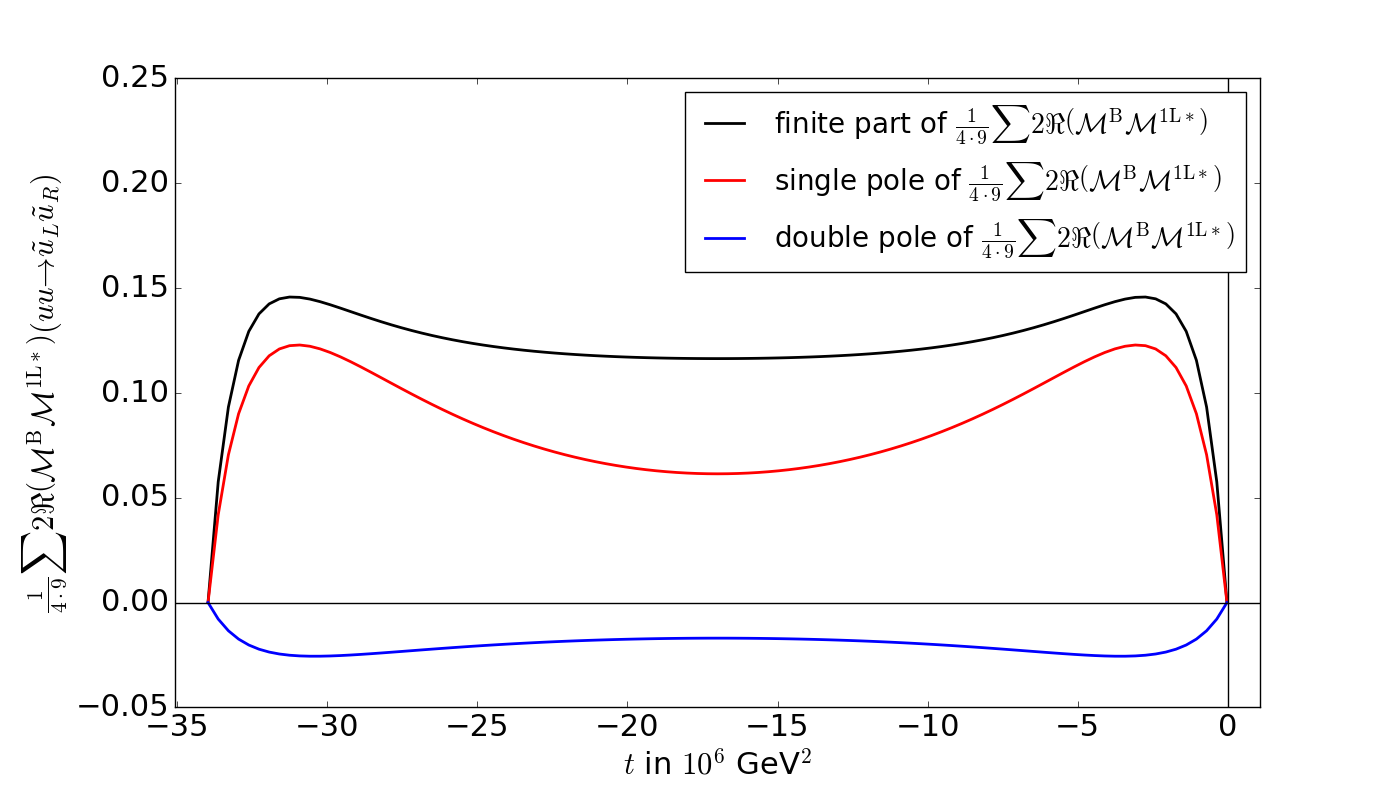
\includegraphics[scale=.5]{figures/MatrixElement_Poles.png}
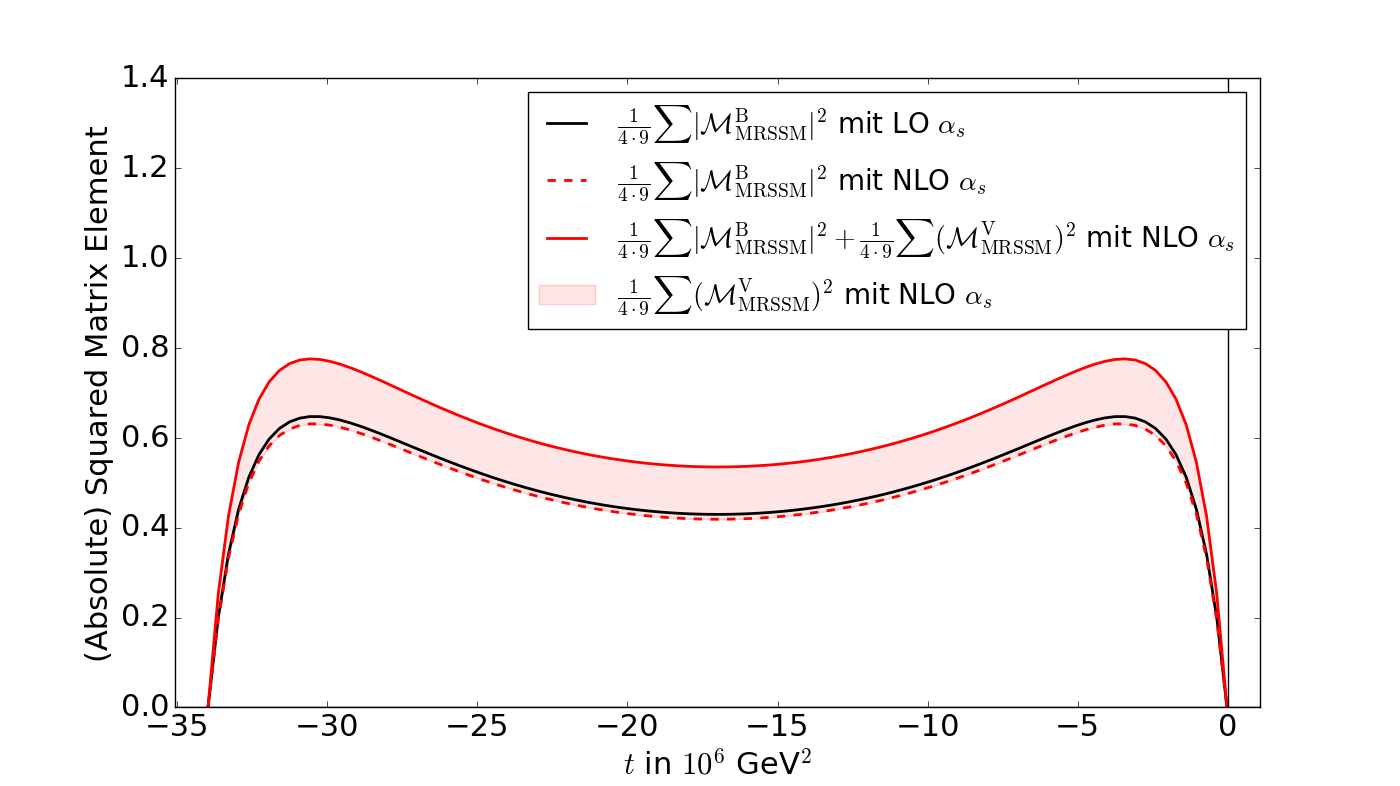
\includegraphics[scale=.5]{figures/MatrixElement.png}
\caption{The figure at the top shows the coefficients of $\mathcal{O}(\epsilon^0)$, $\mathcal{O}(\epsilon^{-1})$ and $\mathcal{O}(\epsilon^{-2})$ terms of the absolute squared matrix element of $uu \to \tilde{u}_L\tilde{u}_R$ in the MRSSM as a function of the Mandelstam variable $t$. External helicities and colors are averaged. The parameters are fixed to $m_{\tilde{q}} = \mu = \unit[1000]{GeV}$, $m_{\tilde{g}} = \unit[2000]{GeV}$, $m_{\sigma} = \unit[5000]{GeV}$ and $\sqrt{s} = \unit[6000]{GeV}$ which is the partnoic center of mass energy.\newline
The figure at the bottom shows the absolute squared matrix element of $uu \to \tilde{u}_L\tilde{u}_R$ in the MRSSM at tree-level with $\alpha_s = $ from the leading order parton density function $\mathtt{MMHT2014}$\cite{Harland-Lang:2014zoa}, and $\alpha_s = $ from the netxt-to-leading order parton density function as well as the contribution from the virtual absolute squared matrix element.}\label{fig:MatrixElement}
\end{center}
\end{figure}